\documentclass{article} % For LaTeX2e
\usepackage{nips15submit_e,times}
\usepackage[colorlinks,linkcolor=red]{hyperref}
\usepackage{url}
\usepackage{amsmath}
\usepackage{graphicx}
\usepackage{float}
\usepackage{bm}
\usepackage{amssymb}
%\documentstyle[nips14submit_09,times,art10]{article} % For LaTeX 2.09


\title{CS499 Homework 9 (First Draft)}


\author{
	Intersteller\thanks{ Use footnote for providing further information
		about author (webpage, alternative address)---\emph{not} for acknowledging
		funding agencies.}
	Department of Computer Science
	Cranberry-Lemon University
	Pittsburgh, PA 15213
}

% The \author macro works with any number of authors. There are two commands
% used to separate the names and addresses of multiple authors: \And and \AND.
%
% Using \And between authors leaves it to \LaTeX{} to determine where to break
% the lines. Using \AND forces a linebreak at that point. So, if \LaTeX{}
% puts 3 of 4 authors names on the first line, and the last on the second
% line, try using \AND instead of \And before the third author name.

\newcommand{\fix}{\marginpar{FIX}}
\newcommand{\new}{\marginpar{NEW}}

\newtheorem{theorem}{}

%\nipsfinalcopy % Uncomment for camera-ready version

\begin{document}
	
	
	\maketitle
	
	
	\textbf{Exercise 9.1}\par
    We define$f_1:\mathbb{N}\rightarrow \mathbb{N}$\par
    $f_1\left(0\right)=0,
    f_1\left(1\right)=1,
    \cdots,
    f_1\left(n\right)=n.
    $\par
    We define $f_2:\mathbb{N}\rightarrow \mathbb{N}^2$ based on this graph:
    \begin{figure}[H]
  	\centering
  	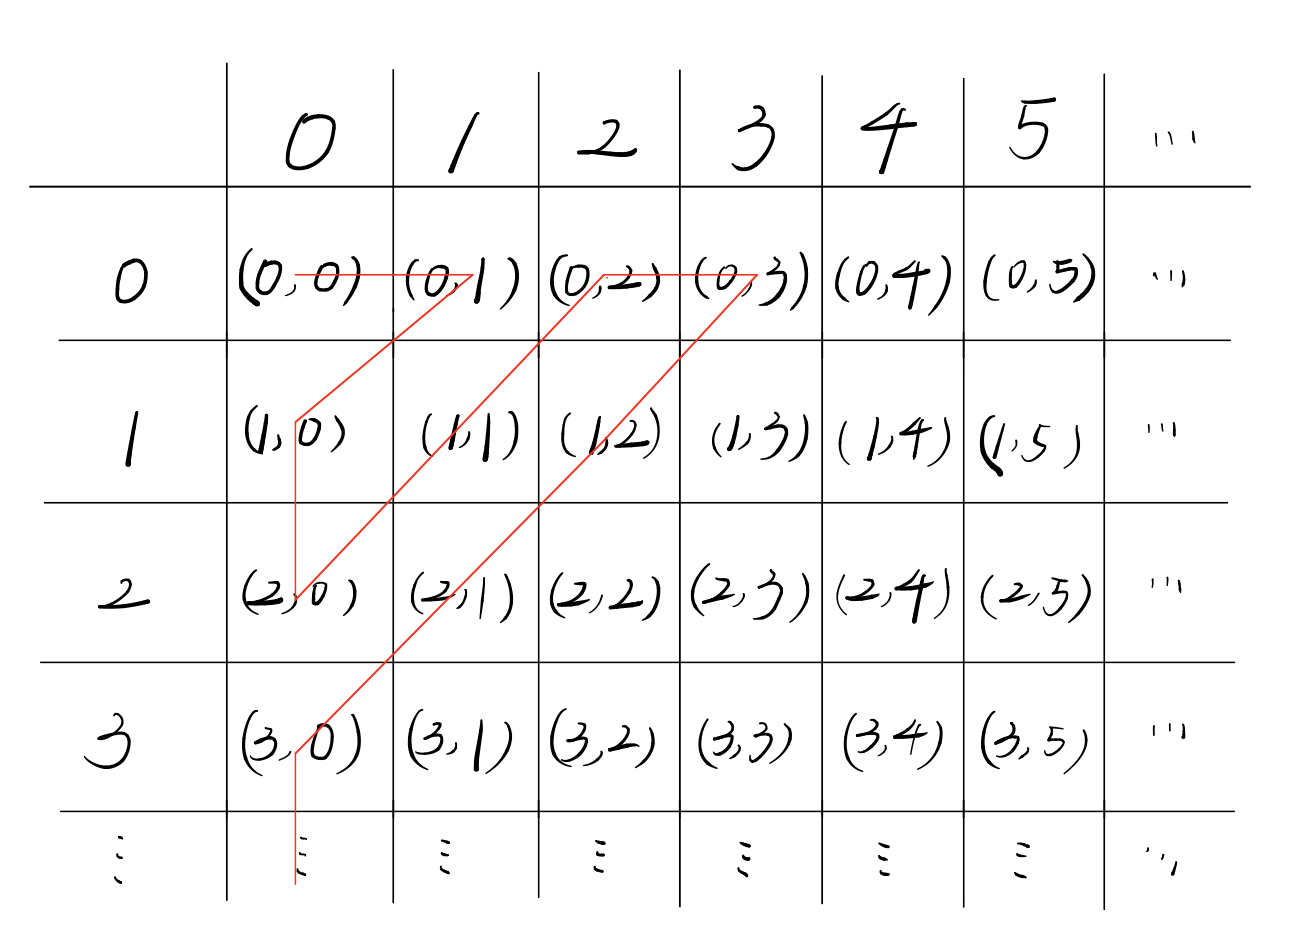
\includegraphics[width=8cm]{9_1_1.png}
  	\caption{}
  	\label{}
  	\end{figure}
    $f_2\left(0\right)=\left(0,0\right),f_2\left(1\right)=\left(0,1\right),f_2\left(2\right)=\left(1,0\right)\cdots$\par
    We define $f_3:\mathbb{N}\rightarrow \mathbb{N}^3$ based on this graph:
   \begin{figure}[H]
  	\centering
  	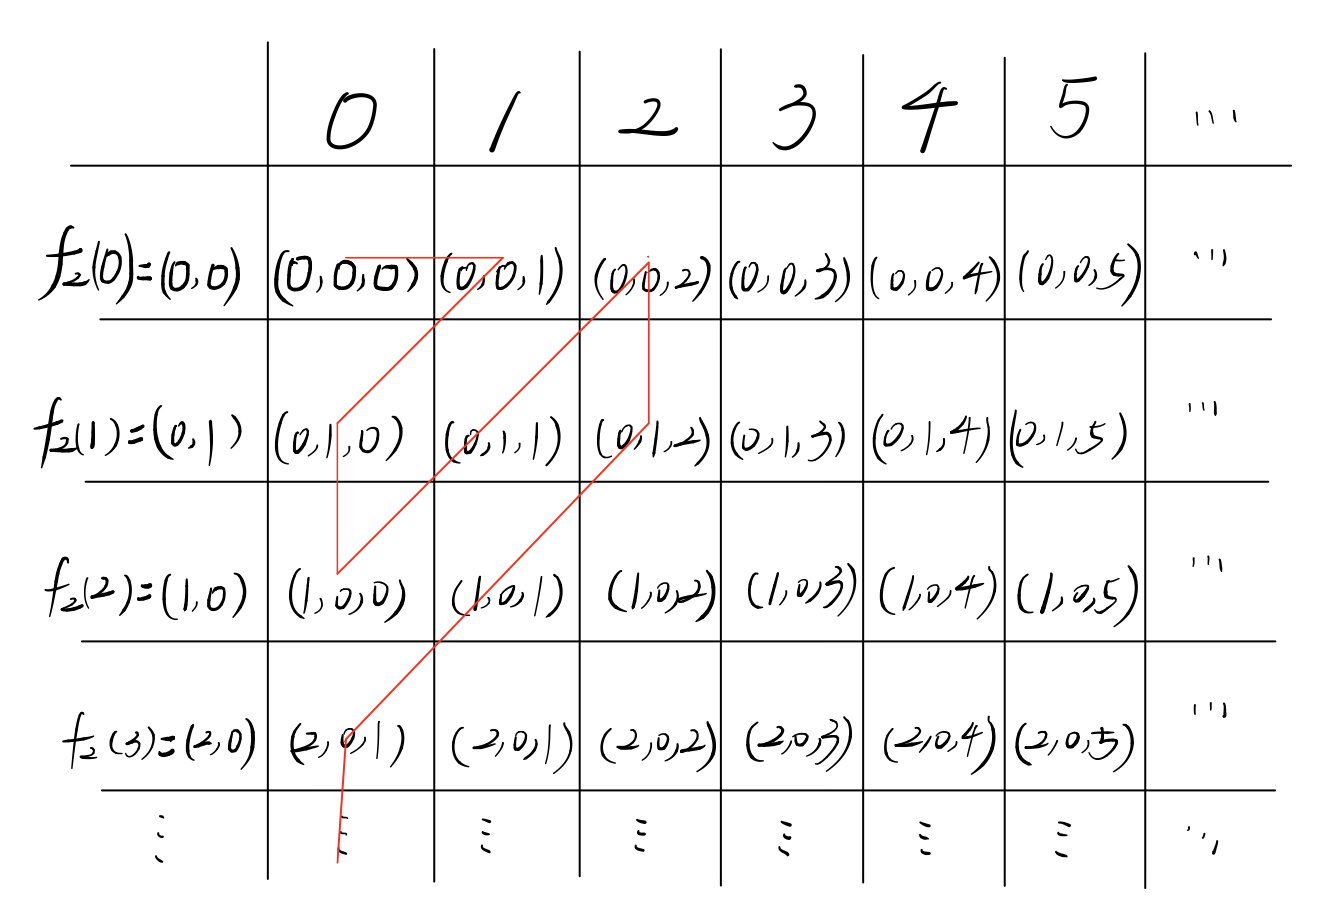
\includegraphics[width=8cm]{9_1_2.png}
  	\caption{}
  	\label{}
  	\end{figure}
    $f_2\left(0\right)=\left(0,0,0\right),f_2\left(1\right)=\left(0,0,1\right),f_2\left(2\right)=\left(0,1,0\right)\cdots$\par
    And so on, we can define $f_k,k\in \mathbb{N}$.
    Now we can define a bijection $\mathbb{N}\rightarrow \mathbb{N}^*$ base on this graph:
    \begin{figure}[H]
  	\centering
  	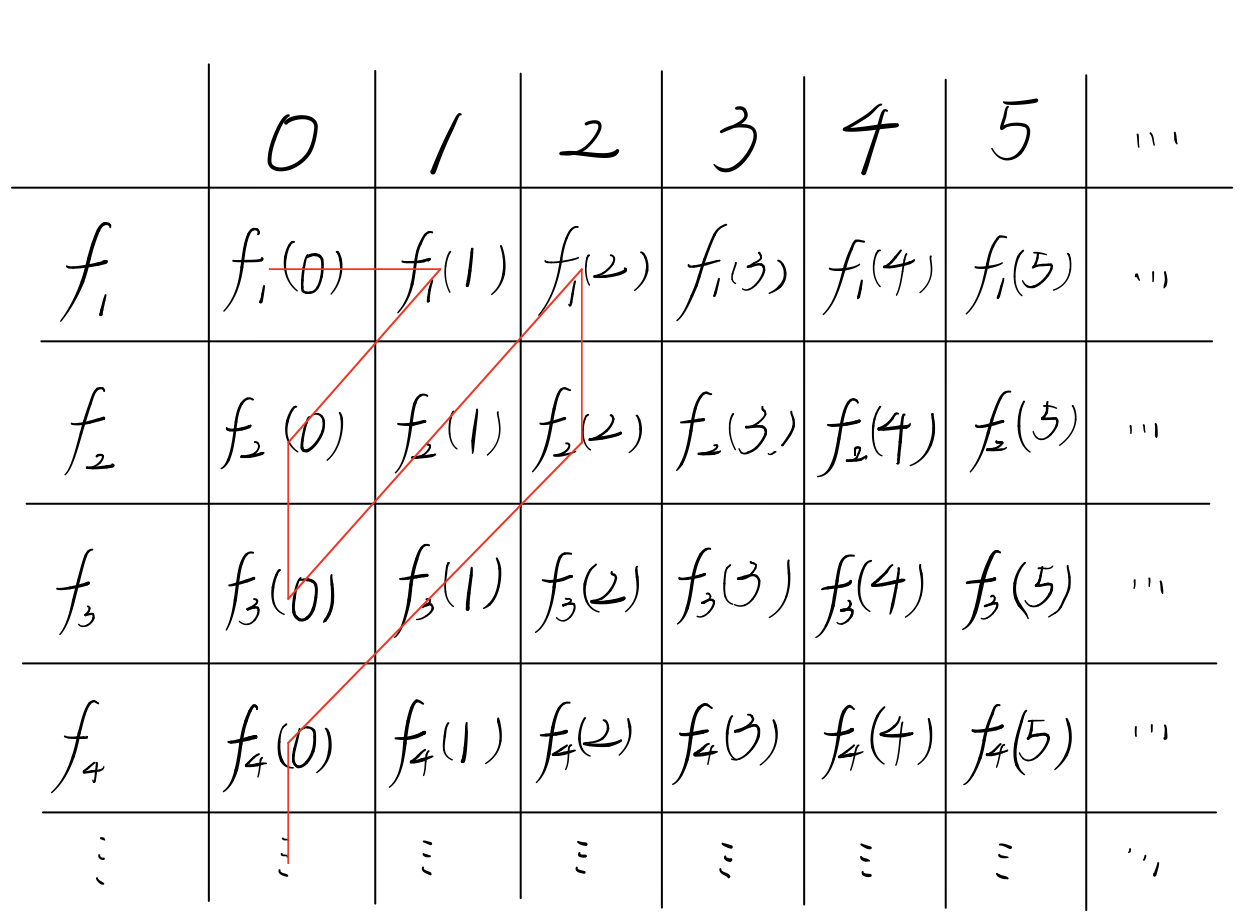
\includegraphics[width=8cm]{9_1_3.png}
  	\caption{}
  	\label{}
  	\end{figure}
    We have $0\rightarrow f_1\left(0\right),1\rightarrow f_1\left(1\right),2\rightarrow f_2\left(0\right)\cdots$. This is a bijection $\mathbb{N}\rightarrow \mathbb{N}^*$.


\textbf{Exercise 9.2}\par
We can define a bijection from $\{0,1\}^\mathbb{N}$ to $\{0,1\}^\mathbb{N}\times \{0,1\}^\mathbb{N}$ as follows.\\
Given $A=(a_1a_2a_3a_4\cdots,b_1b_2b_3b_4\cdots)$, we define $f(A)=a_1b_1a_2b_2a_3b_3a_4b_4\cdots$. To be more precisely, 
$$ f(A)[i]=\left\{
\begin{aligned}
A[1][\frac{i+1}{2}],\ i\ is\ odd\ number \\
A[2][\frac{i}{2}],\ i\ is\ even\ number \\
\end{aligned}
\right.
$$
Obviously, for each $A\in \{0,1\}^\mathbb{N}\times \{0,1\}^\mathbb{N}$, there is only one $f(A)\in \{0,1\}^\mathbb{N}$. For each $B\in \{0,1\}^\mathbb{N}$, there is only one $B=f^{-1}(B)\in \{0,1\}^\mathbb{N}\times \{0,1\}^\mathbb{N}$. Therefore, $f$ is a bijection and $\{0,1\}^\mathbb{N}\cong \{0,1\}^\mathbb{N}\times\{0,1\}^\mathbb{N}$.\\
Using the fact that $\mathbb{R}\cong \{0,1\}^\mathbb{N}$, we can get $\mathbb{R}\cong \mathbb{R}\times \mathbb{R}$.

\textbf{Exercies 9.3}\par
We use the Cantor's method to proove that. For any $A\in (\{0,1\}^\mathbb{N})^\mathbb{N}$, we define that $f(A)$ is the $\{0,1\}^\mathbb{N}$ sequence we get by following the blue line as follows.
 
\begin{figure}[H]
    \centering
    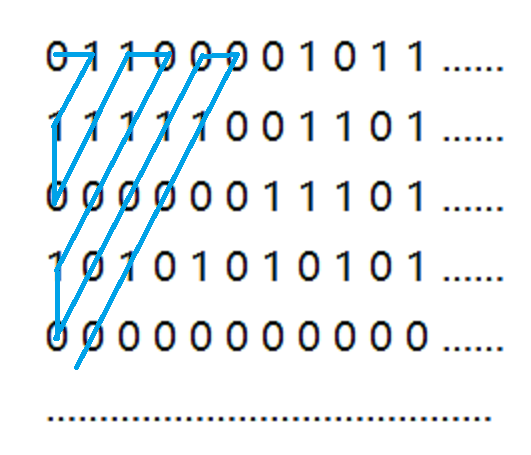
\includegraphics[width=8cm]{9_3_1.png}
    \caption{}
    \label{}
    \end{figure}
It is obvious that for any $B\in \{0,1\}^\mathbb{N}$, we can get to $f^{-1}\in (\{0,1\}^\mathbb{N})^\mathbb{N}$ by writing it down following the blue line. Therefore, $f$ is a bijection and $\{0,1\}\cong (\{0,1\}^\mathbb{N})^\mathbb{N}$. Using the fact that $\mathbb{R}\cong \{0,1\}^\mathbb{N}$, we can get $\mathbb{R}\cong \mathbb{R}^\mathbb{N}$.\par


	\textbf{Exercise 9.4}\par
	We know that one continuous function can be expressed by an infinite sequence of real numbers. 
	Thus we have   $\mathcal{F} \cong \mathbb{R}^{\mathbb{N}}$. According to \textbf{Exercise 9.3},  $\mathbb{R} \cong \mathbb{R}^{\mathbb{N}}$.
	So we have $\mathcal{F} \cong \mathbb{R}^{\mathbb{N}} \cong \mathbb{R}$.\par

	\textbf{Exercise 9.5}\par
    $000\cdots,100\cdots,1100\cdots,11100\cdots$ According to this rule, the first $n$ bits of the $n_{th}$ sequence are $1$, and the remaining bits are $0$. Obviously, these sequences constitute a countably infinite chain.\par
	
	\textbf{Exercise 9.6}\par
	$100\cdots,0100\cdots,00100\cdots,000100\cdots$ According to this rule, the $n_{th}$ bit of the $n_{th}$ sequence is $1$, and the remaining bits are $0$. Obviously, these sequences constitute a countably infinite antichain.\par


	\textbf{Exercise 9.7}\par
    	We can define $A$ using a bijection $f$ from ${\{0,1\}}^{\mathbb{N}}$ to $A$, which is a subset of ${\{0,1\}}^{\mathbb{N}}$ as follows.\\
	Assuming a string $s$ is an element of ${\{0,1\}}^{\mathbb{N}}$ and $f(s)=t$, let $s_k$ determines $t_{2k-1}$ and $t_{2k}$ by the following rule.\\
	If $s_k=0$, then $t_{2k-1}:=0$, $t_{2k}:=1$. If $s_k=1$, then $t_{2k-1}:=1$, $t_{2k}:=0$.\\
	For example:\\
	$$
	s=1011010........
	$$
	$$
	f(s)=10,01,10,10,01,10,01,......
	$$
	Obviously, $f$ is a bijection and $A$ is uncountable. Also, any two elements $t_{a},t_{b}$ of $A$ is not comparable since $"01"$ and $"10"$ is not comparable.
	Thus, $A$ is an required antichain.\par
	\textbf{Exercise 9.8}\par
	 We can define $A$ using a bijection $f$ from $\{0,1\}^{\mathbb{N}}$ to $A$, which is a subset of $\{0,1\}^{\mathbb{N}}$ as follows.\\
 Assuming $s\in \{0,1\}^{\mathbb{N}}$ and $f(s)=t$, the first k digit of $s$ (we call it $s_{1:k}$) determines $t_{(2^{k}+1):(2^{k+1})}$ by the following rule.\\
	 
	 	 Consider the $s_{1:k}$ as a binary number $a_k$, then $t_{(2^{k}+1):(2^{k}+a_k)}:=1$ and the $t_{(2^{k}+a_k+1):(2^{k+1})}:=0$. Specially, we define that the first 2 digits of $t$ are always $0$.\\  
	 
	 For example:\\
	 $$
	 s=1011......
	 $$
	 $$
	 f(s)=00,10,1100,11111000,1111111111100000,......
	 $$
	 Obviously, $f$ is a bijection and A is uncountable. Also, any two elements $t_a,t_b\in A$ is comparable. Assuming that two elements $s_a,s_b$ is different, their first different digit is the $k_{th}$ digit and the $k_{th}$ digit of $s_a$ is 1, then for any $m$ such that $m \ge k$, the binary number of the first m digit of $s_a$ is greater than that of $s_b$, which leads to the conclusion that string $t_a$ is "greater" than $t_b$. Thus, A is the required chain. 

	
\end{document}

